\section{Versuchsaufbau/-durchführung}
Der verwendete Versuchsaufbau ist in Abbildung \ref{fig: aufbau} dargestellt.
\begin{figure}
  \centering
  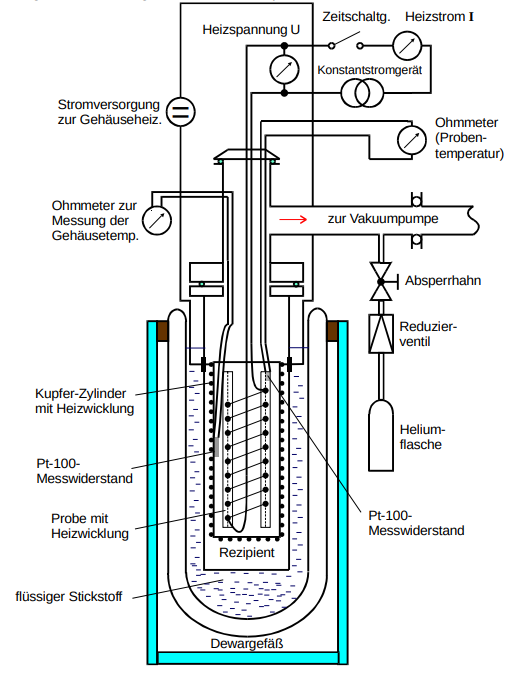
\includegraphics[width = 0.65\textwidth]{./content/images/aufbau.png}
  \caption{Schematische Darstellung des experimentellen Aufbaus des Versuchs V46  \cite{anleitungV47}.}
  \label{fig: aufbau}
\end{figure}
Zunächst wird der in der Darstellung \ref{fig: aufbau} abgebildete Rezipient
mit Hilfe einer Drehschieberpumpe evakuiert. Anschließend wird in den Rezipient
Helium eingefüllt. Mit dem Helium soll verhindert werden, das sich die Restluft
(insbesondere der Stickstoff) im Rezipient verflüssigt oder das sich Wasserkristalle
ausbilden. Der in einem Dewargefäß befindliche Rezipient wird nun mit flüssigen
Stickstoff auf eine Temperatur von ca. $\SI{80}{\kelvin}$ abgekühlt. Ist die
Zieltemperatur erreicht, wird das Helium mit der Drehschieberpumpe abgepumpt und
ein Vakuum erzeugt. Die sich im Rezipienten befindliche Kupferzylinder und
Kupferprobe werden, nach der Evakuierung, langsam erhitzt. Hierbei wurde wahrscheinlich Kupfer als Material
für den Zylinder gewählt, damit dieser dieselbe Emissivität besitzt
wie die Probe. Wie in Abbildung \ref{fig: aufbau} dargestellt, werden für das Erhitzen
Heizwickeln verwendet. Die Temperatur der jeweiligen Heizwickeln kann über jeweils eine
Stromquelle gesteuert werden. Gemesen wird die Temperatur über zwei
Pt-100 Messwiderstände. Bei der Erwärmung der Probe ist darauf zu achten, dass
die Temperaturerhöhung $\Delta T$ lediglich durch die elektrische Energie $E$
der Heizwicklung gegeben ist. Damit lässt sich die Verwendung des Vakuums motiviren -
dieses verhindert näherungsweise die Energieverluste durch Konvektion und
Wärmeleitung. Zusätzlich muss mit Hilfe der beiden Stromquellen sichergestellt
werden, dass die Probe und der Kupferzylinder zu jedem Zeitpunkt die annähernd
selbe Temperatur aufweisen. Hierdurch sollen Verlust durch Wärmestrahlung minimiert werden.
Außerdem kann so näherungsweise eine konstante Temperatur über die gesamte Ausdehnung der Probe
angenommen werden. Somit kann die Temperatur die von dem Pt-100, welches in die Probe eingelassen
ist (vgl. Abb. \ref{fig: aufbau}), gemessen wird stellvertretend für die Temperatur
der gesamten Probe angenommen werden.
Wie schon in dem Kapitel $\ref{sec:theorie}$ erwähnt
ist eine Messung von $C\ua{p}$ experimentell leichter zu realisieren.
Hierzu wird der Temperaturanstieg $\Delta T$ so gewählt, das er, bei
etwa $7-\SI{11}{\degreeCelsius}$ pro $\SI{5}{\minute}$ liegt. Nach dieser Zeit werden die
Widerstände der beiden Pt-100, die Spannung $U$ und Stromstärke $I$ der Probenheizung notiert.
Mit diesen Messdaten, der Probenmasse $m$ und dem Molekulargewicht $M$ lässt sich $C\ua{p}$
berechnen. Hierzu wird der folgende Zusammenhang verwendet:
\begin{equation}
  \label{eq: C_p}
  C\ua{P}=\frac{M \Delta Q}{m\Delta T} = \frac{M}{m}\frac{IU\Delta t}{\Delta T}.
\end{equation}
Das in der Gleichung \eqref{eq: C_p} auftretende $\Delta t$ spiegelt die gewählten $\SI{5}{\minute}$
wieder.
